%===================================== CHAP 4 =================================

\chapter{System Components and implementation}
This chapter will present the different software and hardware components used in this work, in addition to how they are implemented and connected to each other. The two first sections in this chapter will present the hardware and software components respectfully. This is followed by a overview over the components in the \gls{uav} and base station that is used to create the \gls{rtk-gps} system. The two last chapters will explain how the software and hardware implementation respectfully.
\section{Hardware}
The different hardware used in this work is a \gls{uav}, payload computer, \gls{gnss} receiver and antenna.
\subsection{UAV}\label{ss:SkywalkerX8}
The Skywalker X8, see \ref{figure:skywalkerX8}, is a fixed wing \gls{uav} that is moulded out of \gls{epo}, which makes it a cheap and robust platform for prototype testing. The large space within the fuselage makes it ideal for experimental payload and projects with modest requirements.
\begin{figure}[H]
	\centering
		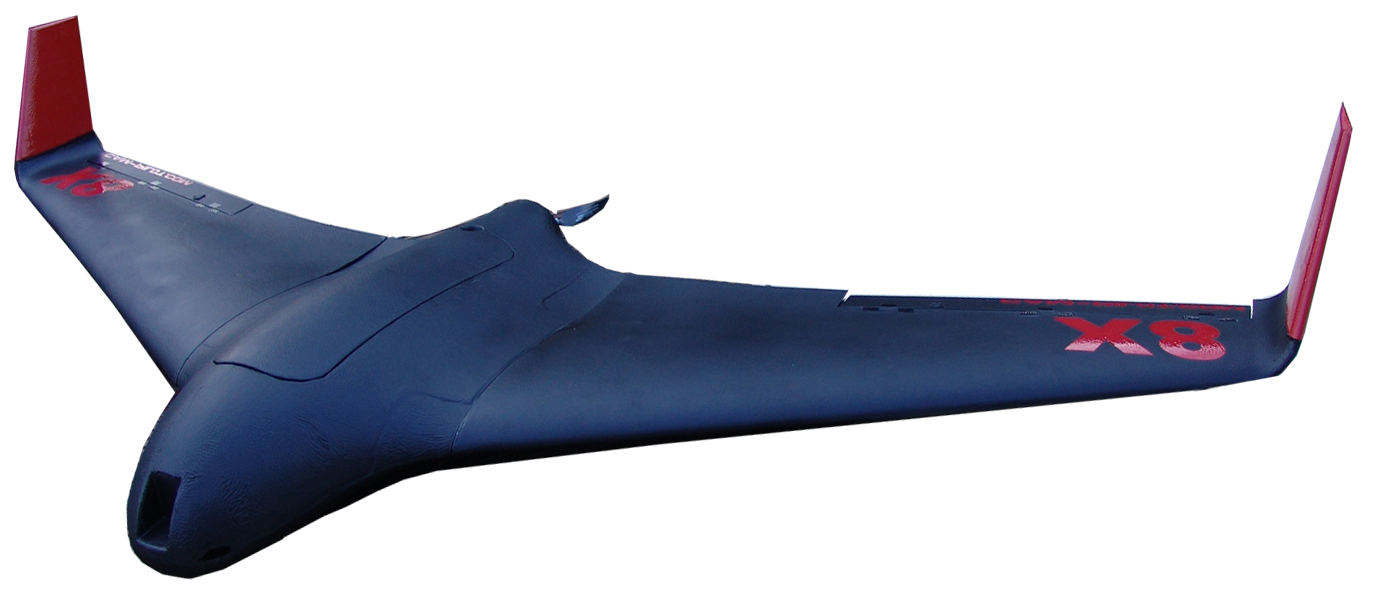
\includegraphics[width=0.7\textwidth]{figs/Wing-X8_white-bgd2.png}
		\caption{X8 Skywalker from Skywalker Technologies, Picture from \url{www.campilot.tv/blog/win-x8}}
		\label{figure:skywalkerX8}
\end{figure}
The X8 has a wingspan of $2120mm$ which allow for a Maximum Take-Off Wight of $4.2kg$, including $1kg$ for the payload. The X8 used in this work is outfitted in according to the specification given in \citep{KlausenX8}. The components that is used in the X8 at the UAVLAB is given in table \ref{tb:X8Components}.
\begin{table}[H]
\begin{center}
\begin{tabular}{l l}
Sensors & 3DR ublox GPS with Compass Kit\\&Pixhawk Airspeed Sensor Kit \\
Servo & Hitec HS-5125MG \\
Motor & Hacker A40 \\
ECU & Jeti Master Spin 66 Pro \\
Main Battery & 1 Zippy Compact 4S 5000 mAh\\
Autopilot & 3DR Pixhawk \\
Primary digital data link & Ubiquiti Rocket M5
\end{tabular}
\end{center}
\caption{Components in the X8 at the UAVLAB}
\label{tb:X8Components}
\end{table}
\subsection{Embedded Computer}
The embedded computer chosen as payload in the X8 is a Beaglebone Black, shown in figure \ref{figure:BeagleBone}. The Beaglebone was chosen because of its sufficient computation power, low energy consumption and variety of communication interfaces. For ease interface access the  the Uavlab at NTNU has developed an extension board called "CAPE".
\begin{figure}[H]
	\centering
		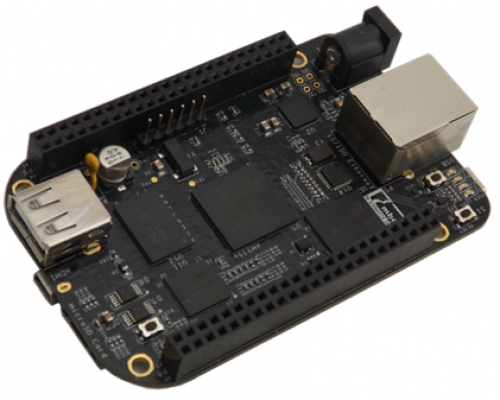
\includegraphics[width=0.7\textwidth]{figs/BeagleBoneBlackE14.png}
		\caption{BeagleBone Black element 14, Picture from \url{http://www.element14.com}}
		\label{figure:BeagleBone}
\end{figure}
The Beaglebone black supports linux operation systems, and is compatiable with the \gls{lsts} toolchain, which will be return to in \ref{S:software}.
\subsection{GNSS receiver}
The system will use two types of \gls{gnss} receivers, namely the Ublox LEA M8T and the Piksi system. 
\subsubsection{Ublox LEA M8T}
The Ublox LEA M8T is a new generation of low-cost \gls{gnss} receiver from ublox. The receiver support sending out raw \gls{gnss} data from both \gls{gps} and \gls{glonass} in the same configuration. The receiver have great performance in acquisition and tracking sensitivity of \gls{gnss} satellites. More technical detalise can be found in  \citep{UbloxDataSheet,UbloxReceiverDescription}.
Write about the Ublox LEA M8T gnss receiver. Also include that it support sending GPS and GLONASS data at the same time. Need to be configured. A receiver were prepare and mounted in the x8.
\begin{figure}[H]
	\centering
		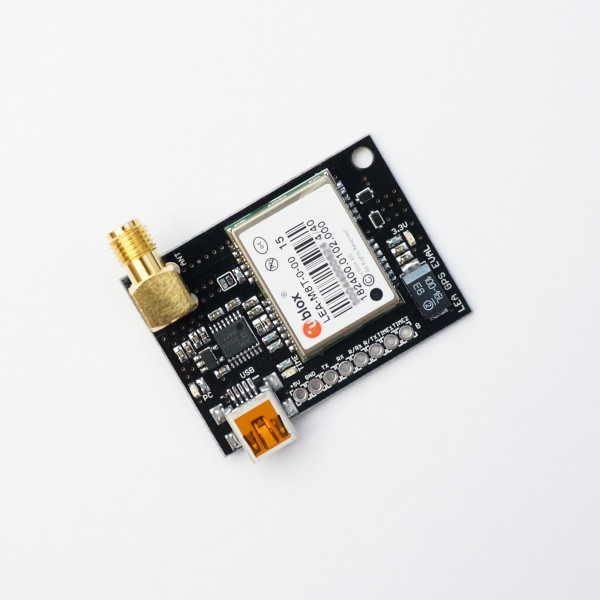
\includegraphics[width=0.7\textwidth]{figs/ubloxLeaM8T.jpg}
		\caption{Ublox LEA M8T, Picture from \url{http://www.csgshop.com}}
		\label{figure:Ublox}
\end{figure}
\subsubsection{Piksi}\label{ss:Piksi}
Piksi, see figure \ref{figure:Piksi}, is a low cost, high performance \gls{gps} receiver with \gls{rtk-gps} functionality with capability for centimeter level relative positioning accuracy developed by Swift Navigation. Piksi is ideal for autonomous vehicles because of its small form factor, fast position solution update rate and low power consumption. 
More detailed information about Piksi can be found in \citep{Piksiv231}
\begin{figure}[H]
	\centering
		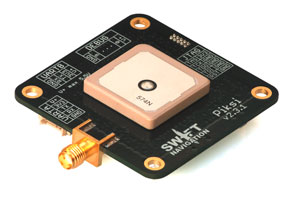
\includegraphics[width=0.7\textwidth]{figs/piksi_top.jpg}
		\caption{Piksi, Picture from \url{www.swiftnav.com}}
		\label{figure:Piksi}
\end{figure}
\subsection{GNSS Antenna}
The navigation system will use two \gls{gnss} antenna, one for the \gls{uav} and the other for the base station. The main criteria for the \gls{uav} antenna is that it's small,compact and have a light weight.

The M1227HTC-A-SMA, seen in figure \ref{figure:Maxtena} has been used in other \gls{uav} setups at the UAVLAB with good results. The antenna is small, compact and with an light weight of $17g$. It's design for L1/L2 gps/glonass bands. Further information or specification can be found in \citep{maxtena}

The base station do not have any restriction on size, weight or aerodynamic. The important factor for a base station antenna is that it has good multipath rejection. Also the base station position should be calculated as accurate as possible which impose further restriction on interference handling, phase center stability and noise rejection.

The Novatel GPS-701-GG, seen i figure \ref{figure:Novatel}, was chosen as the base station antenna. The antenna has excellent multipath rejection whit a highly stable phase center. It has reception for both \gls{gps} and \gls{glonass} \gls{l1} signals..Further information or specification can be found in \citep{novatel}.

\begin{figure}[H]
	\centering
		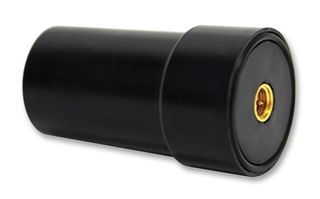
\includegraphics[width=0.7\textwidth]{figs/Maxtena-M1227HCT-A-SMA-image.jpg}
		\caption{Piksi, Picture from \url{http://sigma.octopart.com/21411362/image/Maxtena-M1227HCT-A-SMA.jpg}}
		\label{figure:Maxtena}
\end{figure}

\begin{figure}[H]
	\centering
		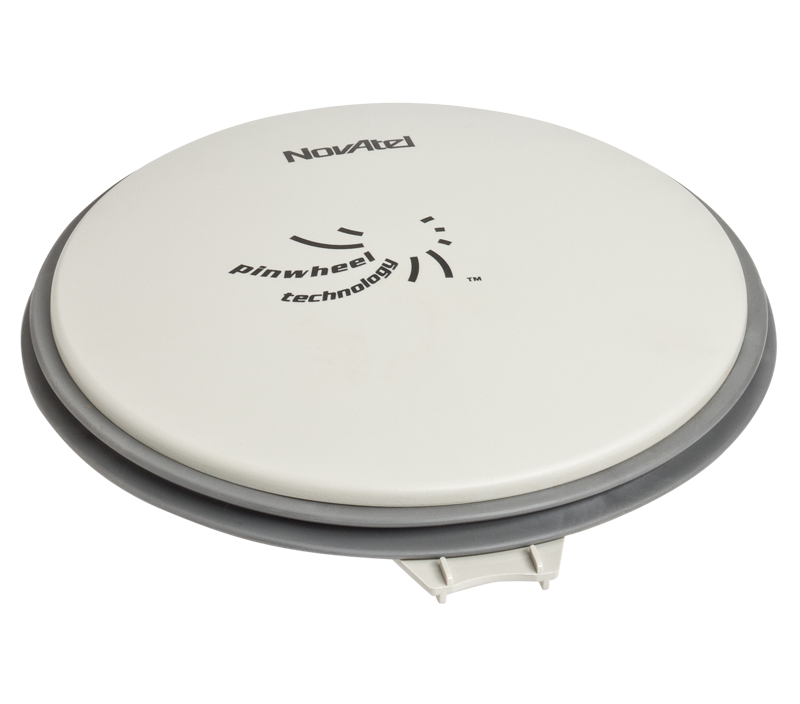
\includegraphics[width=0.7\textwidth]{figs/702-L.png}
		\caption{Piksi, Picture from \url{http://www.novatel.com/assets/Web-Phase-2-2012/Product-Page-Images/Product-Images-Banner-and-Thumbnail/Antennas/702-L.png}}
		\label{figure:Novatel}
\end{figure}


\section{Software}\label{S:software}
This section contain the different software that is used in the x8 system. The following sections contain the operating system that runs on the base station and rover, the middleware used to connect the different tasks, the messages protocol, the missionplaner program and rtklib which will have the main focus.\subsection{GLUED}
Glued is a minimal Linux distribution developed by \gls{lsts}, and design with embedded system in mind. It is platform independent, easy to configure and contain only the necessary packages to run on a embedded system. This makes GLUED a light and fast distribution. GLUED is configured through a single configuration file that which can be created for a specific system. 
\subsection{Dune}
Dune is a runtime environment for unmanned systems on-board software created by \gls{lsts} in Porto, Portugal. The environment type is called a middleware, which is seeing increase usage in unmanned systems. Can refer to ROS or MOOS middleware.

Dune works by setting up individual task that can dispatch and subscribe to different IMC messages. The \gls{imc} messages will be explained in \ref{ss:IMC}
A type of middleware. write how to link rtklib with dune
Refer to the dune wiki page
\subsection{IMC}\label{ss:IMC}
The \gls{imc} protocol that is designed and implemented by \gls{lsts} that is build to interconnect systems of vehicles,sensors and human operators. The protocol is a messages-oriented protocol that enable exchange of real-time information about the environment and updated objectives, such that the participant in the communication can pursue a common goal cooperatively.
\gls{imc} has a standard way of dispatching and consuming messages, which abstracts hardware configuration from the software.

Other feature: Not assuming a specific software architecture, can generate native support for different programming languages and/or computer architectures. Used in network nodes, inter-process and inter thread communication
\subsection{Neptus}
Neptus is an open source command and control software developed by \gls{lsts} for a single or fleet of unmanned vehicles with different types of sensors. The operator can observe real time data from a vehicle, review privios missions and plan future mission. In this work Neptus has been used to extract data logged by Dune during a defined mission, and to monitor the integer ambiguity solution from rtklib and piksi.
\subsection{RTKLIB}\label{ss:Rtklib}
Rtklib is a open source program package for standard and precise positioning with GNSS developed by T. Takasu. Rtklib can use raw GNSS data to estimate the position of the rover. Rtklib can be configured to give a position solution in real time in differential mode. Figure \ref{figure:RTKLIB_STRUCTURE} shows how rtklib can be used in a RTKGNSS mode. The two main moduels here is str2str and rtkrcv. Both will be explalined more closely in the following sections. More information about  rtklib can be found in \citep{Rtklib242}.

\begin{figure}[H]
	\centering
		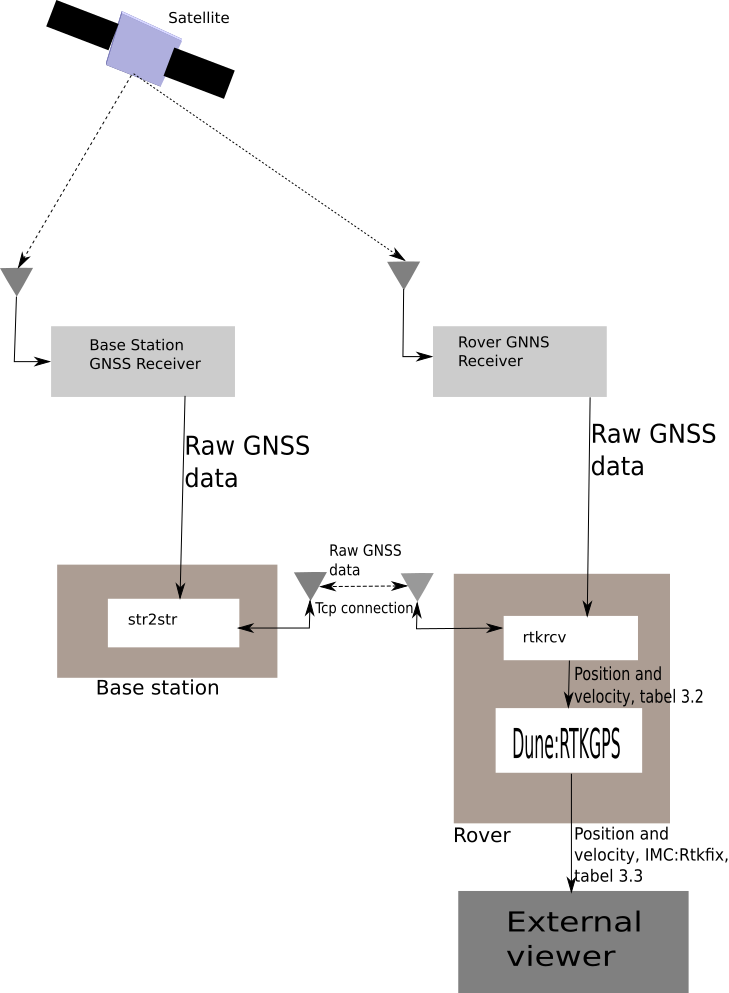
\includegraphics[width=0.7\textwidth]{figs/Rtklib_structure.png}
		\caption{The communication structure of rtklib}
		\label{figure:RTKLIB_STRUCTURE}
\end{figure}
\subsubsection{rtkrcv}
Rtkrcv is the app program that calculate the position of the rover.
Rtkrcv can be configured to have two output streams. The structure of the output stream is given the rtklib manual, however there has been done some alteration in the structure of the output. It's desired in a automatic landing system that have that velocity solution. This is was not provided in the newest version of rtklib, and therefore the source code was altered to send out the velocity data. A quick note here is that it is only available in the output solution is in a enu format. The format of the output is given in table \ref{Tb:RtklibOutput}.

When set configured as a differential GPS rtkrcv uses the LAMBDA method to resolve the integer ambiguity. The solution is considered fixed if the ration between the best estimate and the second best estimate is above a certain threshold.
\begin{table}[!h]
\begin{center}
    \begin{tabular}{ | l | l |}
    \hline
    \textbf{Header} & \textbf{Content} \\ \hline
     1 Time & The epoch time of the solution indicate the true receiver\\& signal reception time. Can have the following format:\\&\\& yyyy/mm/dd HH:MM:SS.SSS:\\& Calender time in GPST, UTC or JST.\\&\\&
     
     WWWW SSSSSSS.SSS:\\&
     GPS week and TOW in seconds  \\ \hline
     2 Receiver Position & The rover receive antenna position \\ \hline
     3 Quality flag (Q) & The flag which indicates the solution quality.\\& 1:Fixed\\& 2:Float\\& 5:Single \\ \hline
     4 Number of valid satellites (ns) & The number of valid satellites for solution estimation. \\ \hline
     5 Standard deviation & The estimated standard deviation of the\\& solution assuming a priori error model and error\\& parameters by the positioning options \\ \hline
     6 Age of differential & The time difference between the observation data epochs\\& of the rover receiver and base station in second. \\ \hline
     7 Ratio factor & The ratio factor of "ratio-test" for standard integer\\& ambiguity validation strategy \\ \hline
     8 Receiver velocity & The velocity of the rover. Given only when output is\\& in enu format \\ \hline
    \end{tabular}
\end{center}
\caption{Rtklib output solution format }
\label{Tb:RtklibOutput}
\end{table}
The position solution is calculated with a Extended Kalman Filter, that can have different structure depending on how rtkrcv is configured
\subsubsection{str2str}
Str2str is the app program that retrieve the ublox signal from the gps and sends over tcp to the rtkrcv app. The str2str is setup to either send RMTC 3 messages, or whatever is send in from the GPS. Since the str2str do not support to send ublox signal directly. How to write that the user should not specify the input format or the output format.


\section{Implementation}
This section explain how the implementation was done for the \gls{rtk-gps} navigation system. Figure \ref{figure:HardSoft} gives an overview on how the system is connected. The implementation includes both a software and a hardware part. 

\begin{figure}[H]
	\centering
		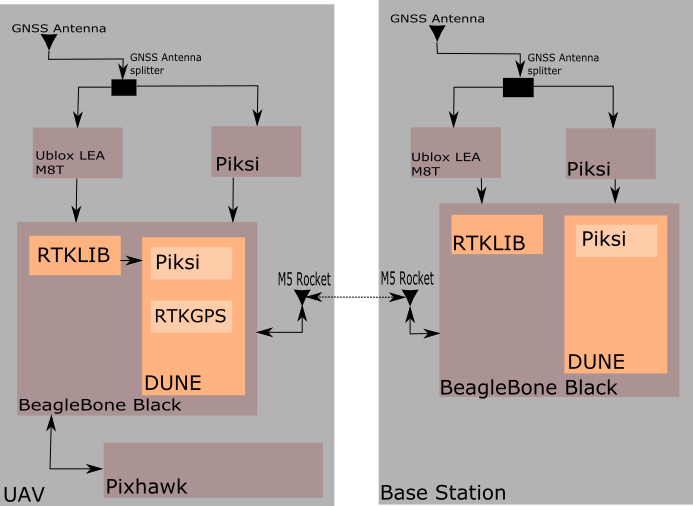
\includegraphics[width=0.7\textwidth]{figs/HardwareSoftware.png}
		\caption{Hardware Software}
		\label{figure:HardSoft}
\end{figure}
\subsection{Software implementation}
The software implementation consist mainly of rtklib and dune. Piksi is also used in the experiment, however it's rtklib and the Dune task RTKGPS that will be discussed thoroughly. It should the noted that the rtklib that is used is an altered version from the latest stable version. The alteration was done in the \gls{enu} output setting where the \gls{enu} velocity variables was included. The new structure is given in \ref{Tb:RtklibOutput}
\subsubsection{Rtkgps}
The \gls{rtk-gps} module in the navigation system consist of three parts. That is rtklib, and the two Dune tasks RTKGPS and Piksi. The RTKGPS task is connected to rtklib though a virtual connection, and the Piksi task has a physical connection to the Piksi receiver.


Rtklib is separated into the base station and the rover. The base station implementation runs the  str2str program were it communicate with the Ublox over a uart cable, and start up a tcp server.

The rover uses the rtkrcv program from rtklib to estimate the position of the rover. Rtkrcv connect itself as a tcp client to the tcp server that str2str create. Rtkrcv is configured in a moving baseline configuration to simulate the behaviour that is expected during a landing on a ship. The configuration file is included in \ref{APPENDIX:RTKLIB}

The output from the Dune tasks is a \gls{imc} message called RtkFix, see table \ref{Tb:RtkFix}, which include the relative position of the \gls{uav} as well as the velocity, type of integer solution and the \gls{gps} \gls{tow}.
\begin{table}[!h]
\begin{center}
    \begin{tabular}{ | l | l |}
    \hline
    \textbf{Header} & \textbf{Content} \\ \hline
     tow & Gps time of Week  \\ \hline
     n & Baseline North coordinate \\ \hline
     e & Baseline East coordinate \\ \hline
     d & Baseline Down coordinate \\ \hline
     v\verb=_=n & Velocity North coordinate \\ \hline
     v\verb=_=e & Velocity East coordinate \\ \hline
     v\verb=_=d & Velocity Down coordinate \\ \hline
     iar\verb=_=hyp & Number of hypotheses in the Integer Ambiguity Resolution \\ \hline
     iar\verb=_=ratio & Quality ratio of Integer Ambiguity Resolution \\ \hline
     type & Type of fix: \\& None = No solution, but RTK task is running
     \\& Obs = No solution, but receiving observations
     \\& Float = Floating point solution of Integer Ambiguity Resolution
     \\& Fix = Fixed(single) solution of Integer Ambiguity Resolution \\ \hline
    \end{tabular}
\end{center}
\caption{The \gls{imc} message RtkFix }
\label{Tb:RtkFix}
\end{table}

\subsection{Hardware implementation}
The base station configuration was already finish by the time this work began. The only hardware that was included was the Ublox and the \gls{gps} antenna splitter. On the \gls{uav} a the payload computer had to be prepared.

The embedded computer uses GLUED as its operating system, and on it runs both Dune and rtklib. The Piksi and Ublox is connected to the BeagleBone over uart cables.

The primary data-link to the \gls{uav} is done with {shf} Ubiquiti AirMax radios, that is based on a Ubiquity Rocket M5

The two \gls{rtk-gps} system is connected to a antenna splitter , figure \ref{figure:AntennaSplitter}, such that both system receive the same \gls{gnss} signals. This is done to easy the comparison of the two \gls{rtk-gps} system, and to remove the antenna as a source of error.

More information on the hardware setup used in the X8 and the Base station is given in \citep{KlausenX8}
\begin{figure}[H]
	\centering
		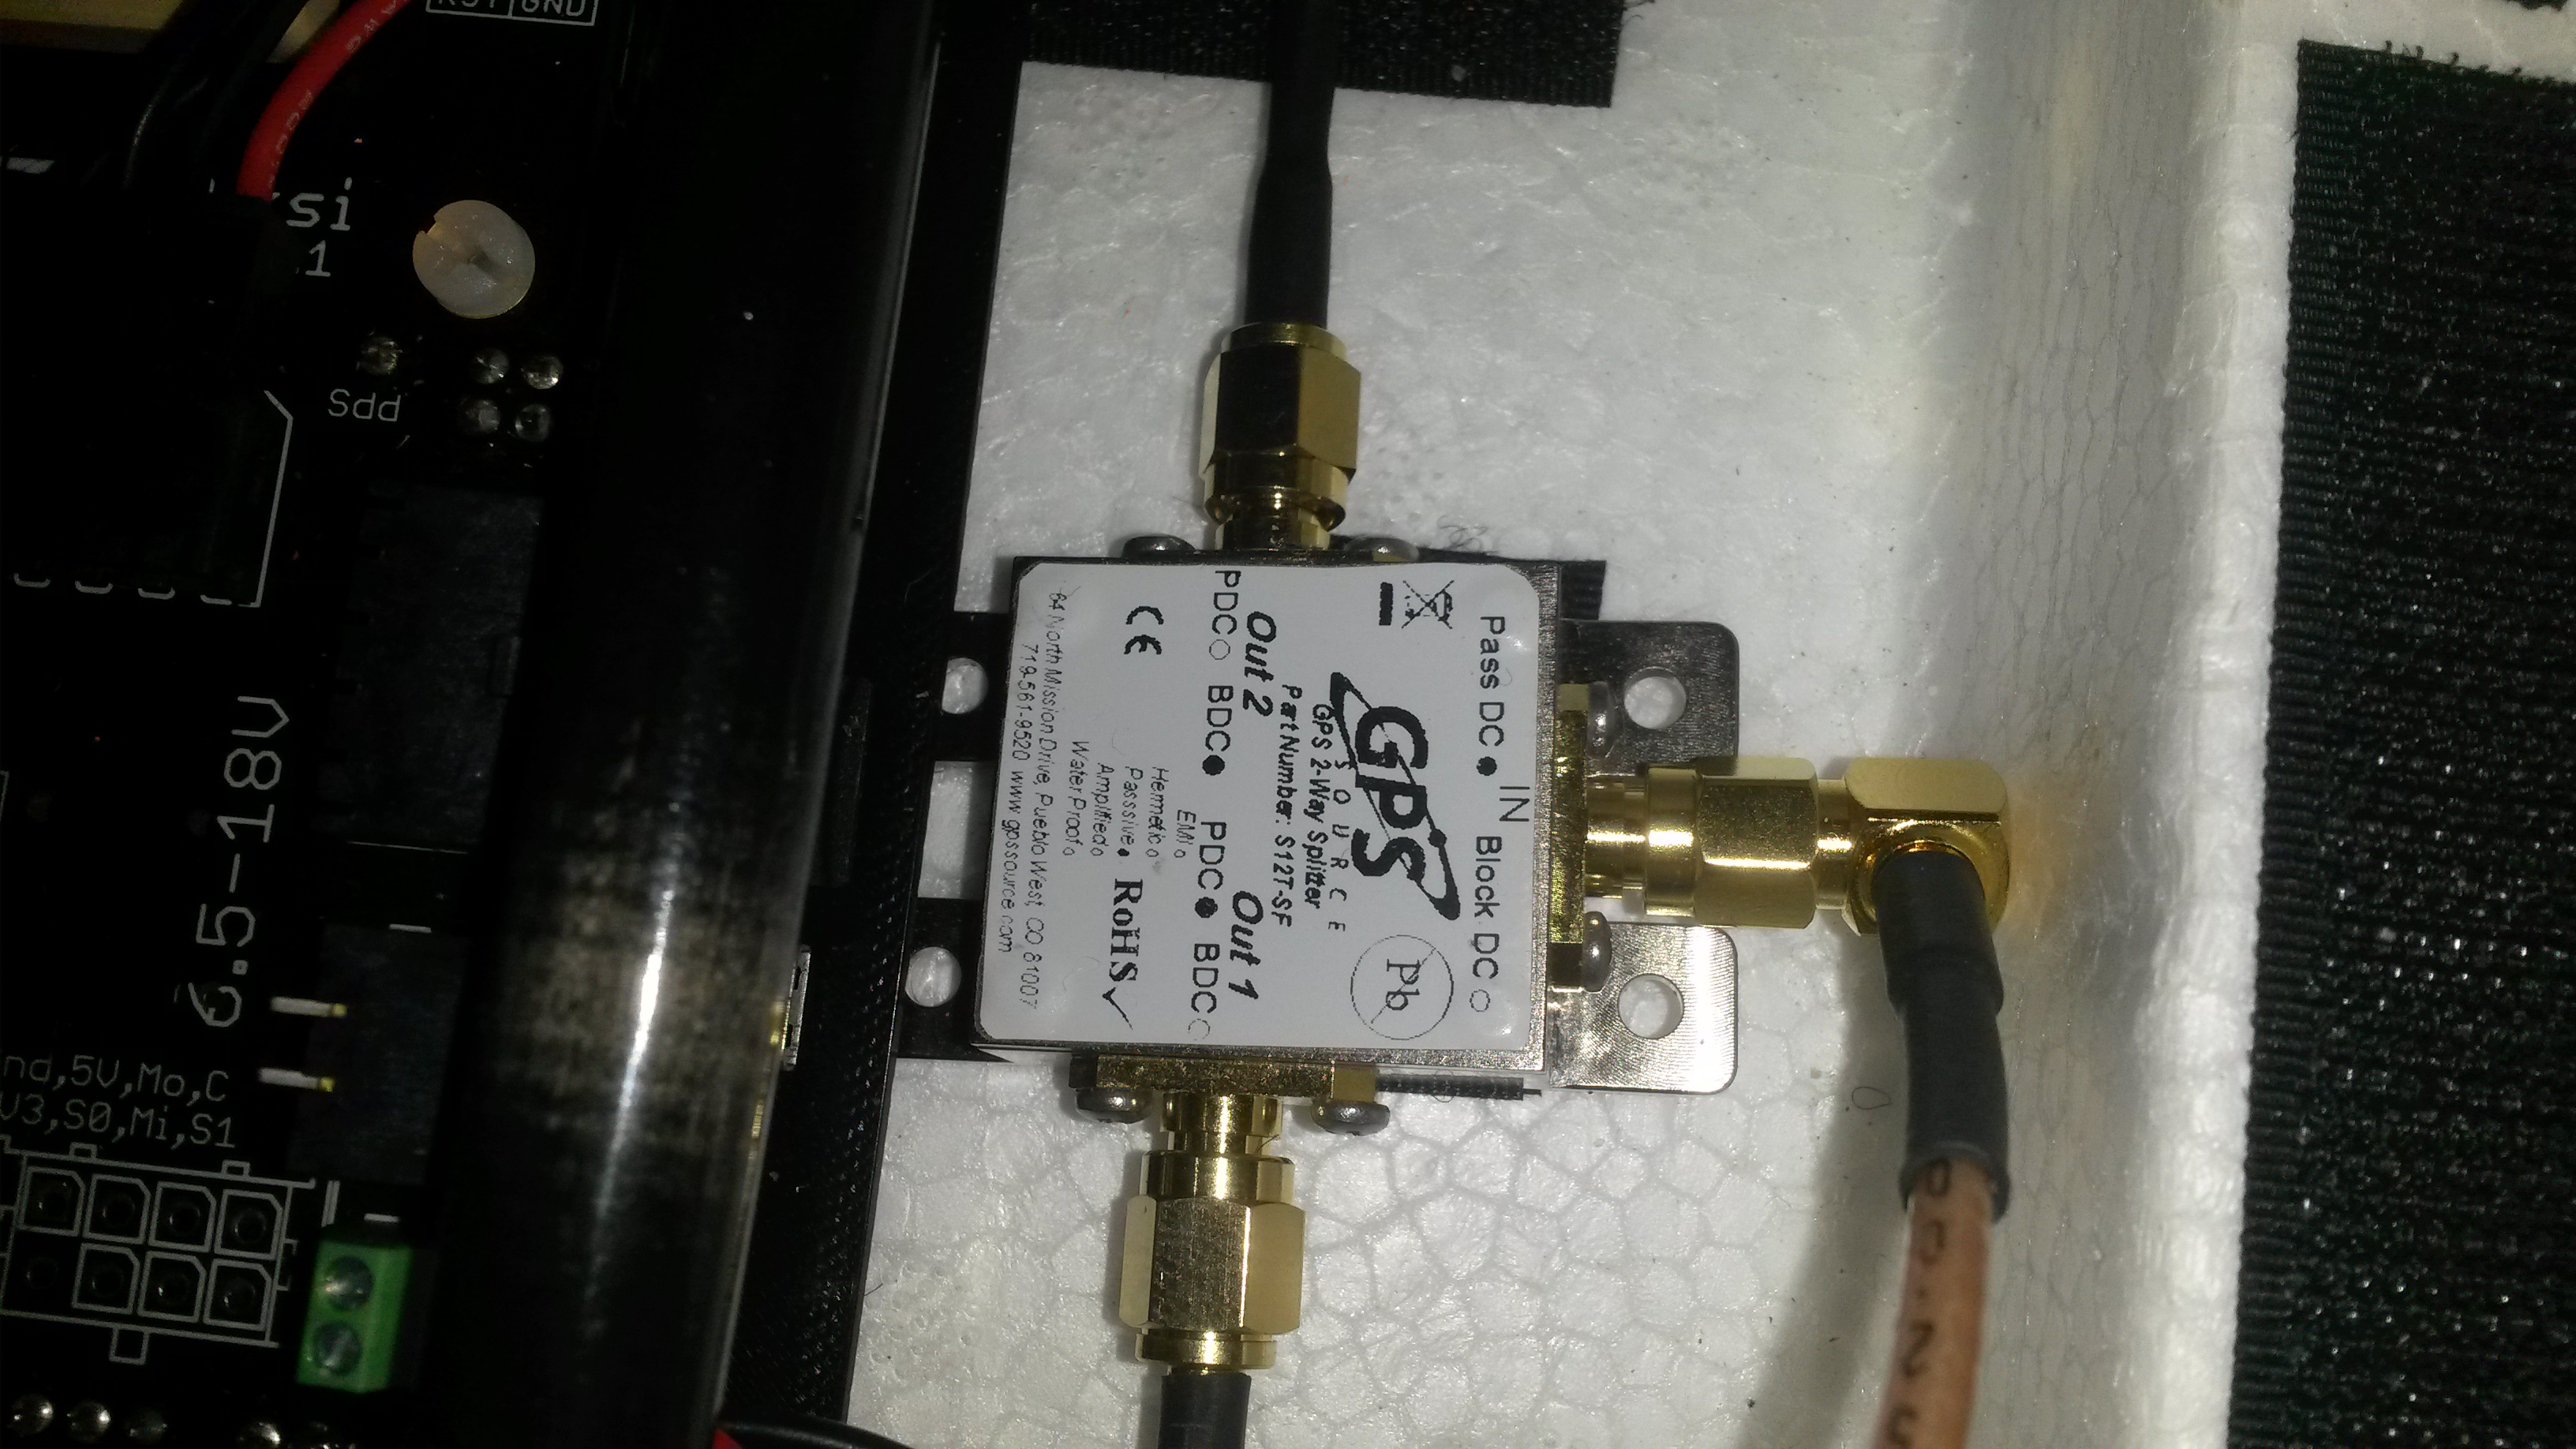
\includegraphics[width=0.7\textwidth]{figs/066.jpg}
		\caption{Antenna splitter}
		\label{figure:AntennaSplitter}
\end{figure}
\cleardoublepage